% DevMPNN-Bench / v2 manuscript -- official NeurIPS 2026 style,
% Evaluations & Datasets track (analysis contribution).
%
% Source of truth: ../paper_v1.md, version converted here = 465 lines,
% MD5 0e00dd407864cc4a685390be4d93e1ef.
%
% Official NeurIPS 2026 style file (neurips_2026.sty from the NeurIPS 2026
% formatting zip). The style sets its own 5.5in x 9in text block, Times/
% Helvetica fonts, loads natbib itself and (in submission mode) adds line
% numbers; we do not override any of that. See CONVERSION_NOTES.md for the
% conversion map and BUILD.md for build instructions.
%
% The Chinese author-facing summary at the top of paper_v1.md is intentionally
% not typeset (the source labels it as a note for the authors); it is kept
% verbatim in AUTHOR_SUMMARY_zh.md.
%
% Author block: in anonymous mode ([eandd] without final/preprint) the style
% prints its own "Anonymous Author(s)" placeholder, so \author is only used for
% local non-anonymous checks such as [preprint,eandd].

\documentclass{article}

% numbered citations; natbib is loaded by the style file
\PassOptionsToPackage{numbers,sort&compress}{natbib}

% official NeurIPS 2026 style, Evaluations & Datasets track, anonymous submission
\usepackage[eandd]{neurips_2026}

\usepackage[utf8]{inputenc}
\usepackage[T1]{fontenc}
\usepackage{amsmath}
\usepackage{amssymb}
\usepackage{bm}
\usepackage{booktabs}
\usepackage{graphicx}
\usepackage{xcolor}
\usepackage{float}          % [H] pinning for the appendix-B tables
\usepackage[hidelinks]{hyperref}

% task-4 page-budget reduction: the style's default caption gap is 7pt.
\setlength{\abovecaptionskip}{2pt}

\graphicspath{{figs/}{../figs/}}

\title{What Developability Benchmarks Do Not Measure: Controllability,
Leakage and Bimodal Failure in Inverse-Folding Evaluation}

\author{Anonymous Author(s)}

\begin{document}

\maketitle

\begin{abstract}
Evaluation practice for developability-oriented inverse folding rests on three
assumptions: that foldability and recovery capture a design method's quality;
that moving a developability property is a property of the model rather than a
dialable control; and that one refolding oracle settles the comparison. We test
all three on the published developability-MPNN family --- ProteinMPNN,
SolubleMPNN, HyperMPNN, MembraneMPNN and LigandMPNN --- plus five plug-and-play
guidance arms, over 35 backbones, 10 arms and 5,936 designs with 5,936 ESMFold
refolds and a second, independent oracle.
We add three measurements that current evaluations do not report: the
\textbf{controllability slope} $k$ (achieved property change per unit of
requested control), \textbf{leakage} (how far unrequested properties drift), and
the \textbf{per-backbone tail} (worst-case behaviour instead of the arm mean).
They show that current practice is measuring the wrong quantity in a way that is
invisible to its own metrics.
Published developability models move surface hydrophobicity by only 4 to 13\%
relative to ProteinMPNN and disagree with each other by 6.0 charge units, yet
standard metrics cannot tell them apart. The controllability slope is
linear and measurable on the full benchmark: $k = -0.010$ surface-apolar
fraction per unit of control strength (per-backbone $R^2 = 0.94$, 35/35
backbones), while the foldability slope is zero to three decimals
($k_{\mathrm{scTM}} = +0.00001$ per unit, $p = 0.98$), so control strength
can be raised tenfold with no measurable cost and the surface property falls
58.6\%. Closed-form guidance on a frozen
ProteinMPNN moves surface hydrophobicity by 32--42\%, aggregation-prone 5-mers
by 42\% and net charge by 10.9 units, with a paired scTM cost whose 95\%
bootstrap CI contains zero for every arm and whose upper bound is 0.028 scTM
(3.4\% relative). Two properties are independently controllable. Leakage is
predictable from the reward weight vector: targeting GRAVY drives net charge
from $+0.2$ to $+20$ while a windowed aggregation reward leaks 0.4 units. The
arm mean is the wrong summary: HyperMPNN differs from ProteinMPNN by $-0.005$
scTM on the median backbone but $-0.064$ on average, because three of
thirty-five backbones collapse by 0.55 to 0.63, and 13 of 35 backbones sit at
ceiling for every arm and cannot discriminate at all. Finally, changing the
oracle shifts absolute scTM by 0.15 and does not preserve the arm ranking
(Spearman $-0.18$ over nine arms), so single-leaderboard reporting is not
defensible.
We release the per-design matrix, aggregate intervals with an explicit minimum
detectable effect of 0.0147 scTM after correction, and a reproduction artifact.
The actionable recommendation is to report control curves and per-backbone
tails rather than arm means, and to state the practical equivalence bound
instead of ``no significant difference''.
\end{abstract}

\section{Introduction}
\label{sec:intro}

Inverse folding is solved well enough to be a commodity: ProteinMPNN~\cite{proteinmpnn}
has 1.66 M parameters (measured from the released weights; the paper reports
1.678 M in its own table), fits on a single A100, and recovers about 52\% of
native residues on its own PDB test set. The bottleneck has moved downstream ---
to whether the designed sequence can actually be made. Solubility, aggregation,
expression and electrostatic behaviour are now the binding constraints in real
campaigns, and the community's answer has been to \textbf{retrain the prior} on
filtered data: SolubleMPNN~\cite{soluble_mpnn} excludes transmembrane entries,
HyperMPNN~\cite{hypermpnn} trains on thermophile structures,
MembraneMPNN~\cite{membranempnn} conditions on a membrane label.

That answer has five consequences for evaluation practice, and this paper
measures each of them. The first three are properties of the models; the last
two are properties of how we evaluate them.

\paragraph{P1 --- single points.}
A retrained model returns one point in property space. There is no knob for
``20\% less hydrophobic than last time'', only a different checkpoint.

\paragraph{P2 --- unreported leakage.}
Moving one property moves others. SolubleMPNN, asked only to remove
transmembrane proteins, also shifts net charge by $-3.5$ units and pI by
$-1.2$. Neither its main text nor the follow-up literature we could find reports
this.

\paragraph{P3 --- blind acceptance metrics.}
Recovery, scTM and pLDDT do not see P2. In our data the six published models,
which disagree by 6.0 charge units, are indistinguishable on every standard
metric (scTM spans 0.78 to 0.88, and the spread is driven by one retrained model
rather than by the property edits).

\paragraph{P4 --- saturation.}
More than a third of the benchmark backbones are at ceiling for every model, so
those cells can only confirm agreement; and because arm differences are bimodal,
the arm mean is dominated by a handful of catastrophic cells. An evaluation that
reports only means therefore cannot tell ``uniformly slightly worse'' from
``fine everywhere except three catastrophic failures''.

\paragraph{P5 --- oracle dependence.}
The comparison is reported against one refolding oracle. We show that a second
oracle shifts absolute scTM by 0.15 and does not preserve the arm ranking, which
makes single-leaderboard reporting an artefact of the choice of oracle rather
than a property of the models.

Our contributions:

\begin{enumerate}
\item \textbf{An evaluation instrument} for control-style design methods: the
  controllability slope $k$, leakage, and the per-backbone tail, each with a
  protocol (backbone as the unit of analysis, paired bootstrap, Holm correction,
  and an explicit minimum detectable effect) that makes negative results
  interpretable.
\item \textbf{A controlled comparison of the whole published
  developability-MPNN family} (ProteinMPNN, SolubleMPNN, HyperMPNN,
  MembraneMPNN, LigandMPNN) against jointly-scored guidance arms on 35 backbones
  and 5,936 designs, with a second oracle.
\item \textbf{Five findings about current practice}, each tied to a measured
  failure: 4--13\% property movement, 6.0 units of inter-model disagreement
  invisible to standard metrics, bimodal tail behaviour hidden by means, a third
  of the benchmark saturated, and a ranking that does not survive a change of
  oracle. Two further results follow from measuring control on the full
  benchmark: the control-folding frontier is flat over a tenfold range of control
  strength, and the position-specific part of the reward is load-bearing (a
  global penalty controls the target better but costs 0.033 scTM and leaks
  charge).
\item \textbf{A closed-form guidance baseline}: for composition-linear
  properties the any-order-autoregressive guidance of
  ProteinGuide~\cite{proteinguide} reduces to a constant per-amino-acid logit
  bias, so a frozen ProteinMPNN becomes a calibrated, reversible knob at no
  extra predictor cost --- the cheapest possible control method, used here as
  the instrument that exposes what the published models' single points cannot
  show.
\end{enumerate}

\textbf{What is and is not new here.} The any-order-autoregressive guidance
identity is due to ProteinGuide~\cite{discrete_guidance,proteinguide} (Nisonoff
et al., 2025; Xiong et al., 2026); we do not claim it. Our contribution is (i)
the closed-form specialisation to composition-linear rewards, which needs no
property predictor at inference time, and (ii) the benchmark that measures what
such control costs, including the leakage and per-backbone analyses. Guidance
through a learned predictor for non-linear objectives (the TAG route in
ProteinGuide) is deliberately out of scope and is listed in the limitations; a
reader should not read this paper as a comparison of guidance algorithms.

\section{Related work}
\label{sec:related}

\paragraph{Inverse folding.}
Structured Transformer~\cite{struc_transformer} (2019) introduced the kNN graph
+ autoregressive formulation; GVP-GNN~\cite{gvp} (2021) added geometric vector
perceptrons; ProteinMPNN~\cite{proteinmpnn} (2022) simplified to a
message-passing encoder--decoder with a \emph{random decoding order} and became
the field's default; ESM-IF1~\cite{esm_if1} (2022) showed that 12 M AlphaFold2
structures buy more than architecture (+9.4 pp over GVP-GNN, and +13.3 pp over
the same architecture trained on CATH only in our reading of its tables);
PiFold~\cite{pifold} (2023)
decodes in one shot; LigandMPNN~\cite{ligandmpnn} (2025) conditions on atomic
context. All of these are evaluated on recovery and scTM; none measures
controllability.

\paragraph{Developability-oriented design.}
SolubleMPNN~\cite{soluble_mpnn} (2024) retrains ProteinMPNN on the same PDB
snapshot minus 17,369 transmembrane entries; HyperMPNN~\cite{hypermpnn} (2024)
retrains on thermophile AF2 structures and, in its own measurements, pays a
large expression tax (soluble yield 0.4 vs 25.8 mg/L for the parent model);
MembraneMPNN~\cite{membranempnn} ships conditioned weights
without a paper. Their common structure is a \textbf{prior shift}, which is
irreversible and leaks into every property at once.

\paragraph{Inference-time control.}
Classifier guidance, classifier-free guidance, SMC/Feynman--Kac particle
steering (applied to RFdiffusion in 2025~\cite{fk_rfdiffusion}), and
plug-and-play discrete guidance (ProteinGuide,
2025~\cite{discrete_guidance,proteinguide}) whose AA-ARM update is
\[
  \tilde{p}(x_i{=}a \mid x_S) \;\propto\;
  p_\theta(a \mid x_S)
  \left[
    \frac{p(y \mid x_S \cup a)}{p(y \mid x_S)}
  \right]^{\gamma}.
\]
ZetaDial (2026)~\cite{zetadial} is the closest protein work: a global charge
bias solved per protein, reported to collapse foldability at strong tilt. No
work compares this family against retrained developability models under one
protocol.

\paragraph{Benchmarks.}
ProteinInvBench~\cite{proteininvbench} (NeurIPS 2023 D\&B) standardises
single-chain, multi-chain and de novo tasks; MotifBench~\cite{motifbench} (2025)
standardises motif scaffolding; ProteinGym~\cite{proteingym} and
FLIP~\cite{flip} cover sequence--function. None measures \emph{whether a model
can be steered}, which is the gap this benchmark fills.

\section{Benchmark design}
\label{sec:method}

\subsection{Backbones}
\label{sec:backbones}

35 monomeric PDB entries, chain A, 56--415 residues, downloaded and validated
by \texttt{prep\_targets.py} (CA count 50--450, parseable chain A). The list is
fixed in \texttt{data/targets30.txt} so that future arms cannot change the
problem set.

The composition of the set --- length distribution, experimental method and
resolution --- is tabulated in Table~\ref{tab:backbones} in the appendix.

The set is deliberately broad in fold space but \textbf{skewed small} (more
than half are under 100 residues), which matches the monomer regime where
inverse folding is usually benchmarked but not the 150--300 residue range that
dominates real design campaigns. Five NMR entries are included because they are
standard small-monomer benchmarks; ProteinMPNN is known to recover native
sequences poorly on NMR structures, and those backbones contribute some of the
low-scTM cells in every arm. Both points are revisited in the limitations.

\subsection{Arms}
\label{sec:arms}

\begin{table}[htbp]
  \centering
  \small
  \begin{tabular}{@{}llp{2.2in}@{}}
    \toprule
    Family & Arm & Mechanism \\
    \midrule
    published & ProteinMPNN \texttt{v\_48\_020} & baseline (a seed-1 replicate is run only to measure repeatability, and is not an arm) \\
    published & SolubleMPNN \texttt{v\_48\_020} & retrained without transmembrane entries \\
    published & HyperMPNN \texttt{v48\_020\_epoch300\_hyper} & retrained on thermophile AlphaFold2 structures \\
    published & MembraneMPNN global-label, fed ``soluble'' & conditioned input \\
    published & LigandMPNN \texttt{v\_32\_020} on backbone atoms & extra atom-context encoder \\
    guided & surf $\lambda$10 & per-residue apolar penalty on exposed sites \\
    guided & agg $\lambda$10 & windowed (5-residue) exposed apolar penalty \\
    guided & charge $\lambda{+}3$ & constant per-AA charge tilt \\
    guided & surf10 / charge$-2$ & two-property tilt (acidic branch) \\
    guided & surf10 / charge$+2$ & two-property tilt (basic branch) \\
    \bottomrule
  \end{tabular}
  \caption{Benchmark arms and their mechanisms.}
  \label{tab:arms}
\end{table}

Sixteen designs per (arm, backbone), temperature 0.1, fixed seed. The main
table below is this 16-design run; a predecessor run at 8 designs per cell is
kept in \texttt{results/AGGREGATE.md} and is used only for the temperature
ablation.

\subsection{Guidance: the AO-ARM closed form}
\label{sec:guidance}

ProteinMPNN samples residues in a random order and conditions on any subset of
known positions, i.e.\ it \emph{is} an any-order autoregressive model.
ProteinGuide's update for AO-ARMs multiplies the per-position categorical by a
likelihood ratio. For a property that is linear in amino-acid composition,
$\phi(a)=\sum_a n_a w_a$, that ratio is position-independent:
\[
  \log \tilde{p}(x_i{=}a \mid x_S)
  = \log p_\theta(a \mid x_S) - \lambda \cdot w_a + \mathrm{const},
\]
so guidance is \textbf{exactly} a constant per-amino-acid logit bias --- no
predictor calls, no approximation. ProteinMPNN's sampler computes
\texttt{softmax(logits/T + bias/T)}, hence we store $b = \lambda T$ to obtain an
effective logit shift $\lambda$. Surface hydrophobicity uses a per-residue
version, $b_{i,a} = -\lambda \cdot h_a \cdot s_i$, where $s_i \in \{0,1\}$
marks exposure computed from the \textbf{input backbone} (C$\alpha$ neighbour
count, median split), never from the design. Multi-property arms add the biases.

\paragraph{Boundary.}
Non-linear or neighbour-dependent objectives (aggregation patches beyond the
windowed proxy, $\pi$-stacking, stability) need ProteinGuide's TAG approximation
and are out of scope here.

\subsection{Metrics}
\label{sec:metrics}

\begin{itemize}
\item \textbf{scTM}: TM-score of the ESMFold-refolded design~\cite{esmfold}
  against the input backbone, at valid sites.
\item \textbf{recovery}: identity to the native sequence.
\item \textbf{diversity}: mean pairwise Hamming within the design set of one
  (arm, backbone) cell (16 designs in the main run, 8 in the \S4.1b ablation).
\item \textbf{controllability slope $k$}: OLS slope of achieved property on
  requested $\lambda$.
\item \textbf{leakage}: $\sum_{j\neq\mathrm{target}} |\Delta\phi_j|$
  normalised by $|\Delta\phi_{\mathrm{target}}|$.
\end{itemize}

\subsection{Statistical protocol}
\label{sec:stats}

Unit of analysis is the \textbf{backbone}, never the design. For every arm
comparison we form per-backbone means, then a paired bootstrap over backbones
($B = 10{,}000$) and report the 95\% percentile interval. Repeatability is
estimated by re-running ProteinMPNN with a different sampling seed on all 35
backbones (same weights, same temperature), which bounds the resolution of
every comparison. Designs are never pooled across backbones. Nine comparisons are made
against one baseline, so we report raw bootstrap $p$-values \textbf{and}
Holm-adjusted $p$-values and treat an effect as confirmed only if it survives
Holm at $\alpha = 0.05$.

\textbf{Power.} The seed-1 replicate gives the paired per-backbone standard
deviation of a null comparison directly, sd = 0.0240 scTM over 35 backbones.
With that dispersion the minimum detectable effect at 80\% power is
\textbf{0.0114 scTM (1.35\% relative)} for a single uncorrected comparison and
\textbf{0.0147 scTM (1.74\%)} once the Holm threshold for nine comparisons is
applied. This number is the honest interpretation of every null result in this
paper: the data exclude effects larger than about 0.015 scTM, not effects of
zero. It also explains why the guided arms' point estimates ($+0.003$ to
$+0.009$) cannot be called improvements, and why HyperMPNN's $-0.064$, which is
four times the corrected threshold, is the only effect of a size this benchmark
can resolve.

\section{Results}
\label{sec:results}

\subsection{Main table (35 backbones, 5,936 designs)}
\label{sec:main-table}

% Figure numbers follow the numbering assigned in the markdown source
% (Figure 2 appears in Section 4.1, Figure 1 in Section 4.2). The counters
% are set explicitly so that the compiled paper keeps the same number for
% each figure.
\setcounter{figure}{1}

\begin{table*}[htbp]
  \centering
  \scriptsize
  \setlength{\tabcolsep}{2pt}
  \begin{tabular}{@{}lrrrrrrrr@{}}
    \toprule
    Arm & n & surface apolar & aggregation 5-mer & net charge & pI & recovery & diversity & \textbf{scTM} \\
    \midrule
    ProteinMPNN & 560 & 0.430 & 0.212 & $+1.95$ & 7.87 & 0.436 & 0.283 & 0.8444 \\
    ProteinMPNN (seed 1) & 560 & 0.434 & 0.212 & $+1.89$ & 7.82 & 0.437 & 0.288 & 0.8434 \\
    SolubleMPNN & 560 & 0.378 & 0.168 & $-1.57$ & 6.64 & 0.425 & 0.283 & 0.8457 \\
    HyperMPNN & 560 & 0.411 & 0.213 & $+4.30$ & 8.40 & $\bm{0.376}$ & 0.258 & $\bm{0.7809}$ \\
    MembraneMPNN (global) & 528 & 0.376 & 0.178 & $+0.30$ & 7.49 & 0.439 & 0.288 & 0.8748 \\
    LigandMPNN & 528 & 0.397 & 0.176 & $-1.00$ & 6.64 & 0.443 & 0.263 & 0.8717 \\
    guide surf $\lambda$10 & 528 & $\bm{0.259}$ & 0.120 & $+1.72$ & 7.87 & 0.446 & 0.272 & 0.8703 \\
    guide agg $\lambda$10 & 528 & 0.291 & $\bm{0.124}$ & $\bm{+1.96}$ & 7.97 & 0.448 & 0.280 & $\bm{0.8718}$ \\
    guide charge $\lambda{+}3$ & 528 & 0.413 & 0.206 & $\bm{-8.52}$ & 5.35 & 0.456 & 0.277 & 0.8618 \\
    guide surf10/charge$-2$ & 528 & 0.250 & 0.112 & $\bm{+12.83}$ & 9.94 & 0.444 & 0.276 & 0.8726 \\
    guide surf10/charge$+2$ & 528 & 0.258 & 0.120 & $\bm{-8.70}$ & 5.57 & 0.448 & 0.266 & 0.8671 \\
    \bottomrule
  \end{tabular}
  \caption{Main table (35 backbones, 5{,}936 designs).}
  \label{tab:main}
\end{table*}

Folded backbones per arm: 35 for ProteinMPNN/SolubleMPNN/HyperMPNN, 33 for
MembraneMPNN/LigandMPNN and the guided arms (two backbones failed to sample for
those arms). All comparisons are paired, so the differing counts do not affect
the intervals.

\paragraph{Repeatability.}
Seed 0 $\to$ seed 1, same weights and temperature: $\Delta$scTM =
$\bm{-0.0010}$, 95\% CI $[-0.0086, +0.0076]$ (35 backbones). This $\pm 0.008$
band is the resolution floor of the benchmark and the reason every comparison
below is paired.

\begin{table*}[htbp]
  \centering
  \scriptsize
  \setlength{\tabcolsep}{2pt}
  \begin{tabular}{@{}lllllp{1.0in}l@{}}
    \toprule
    Arm & $\Delta$scTM & CI & $p$ (raw) & $p$ (Holm) & targeted change & leakage \\
    \midrule
    SolubleMPNN & $+0.0013$ & $[-0.0118, +0.0169]$ & 0.89 & 1.00 & surface $-12.1$\% & charge $-3.5$ \\
    \textbf{HyperMPNN} & $\bm{-0.0635}$ & $\bm{[-0.1259, -0.0117]}$ & $\bm{0.006}$ & $\bm{0.057}$ & surface $-4.4$\% & charge $+2.4$ \\
    MembraneMPNN (global) & $+0.0207$ & $[-0.0013, +0.0561]$ & 0.096 & 0.76 & surface $-12.6$\% & charge $-1.7$ \\
    LigandMPNN & $+0.0176$ & $[-0.0033, +0.0513]$ & 0.21 & 1.00 & surface $-7.7$\% & charge $-3.0$ \\
    \textbf{guide surf $\lambda$10} & $+0.0066$ & $[-0.0054, +0.0215]$ & 0.34 & 1.00 & surface $\bm{-39.8\%}$ & charge $-0.2$ \\
    \textbf{guide agg $\lambda$10} & $+0.0081$ & $[-0.0020, +0.0216]$ & 0.16 & 1.00 & aggregation $\bm{-42\%}$ & charge 0.0 \\
    guide charge $\lambda{+}3$ & $-0.0019$ & $[-0.0100, +0.0069]$ & 0.63 & 1.00 & charge $\bm{-10.5}$ & surface $-4.0$\% \\
    guide surf10/charge$-2$ & $+0.0089$ & $[-0.0057, +0.0278]$ & 0.30 & 1.00 & surface $-41.9$\%, \newline charge $+10.9$ & --- \\
    guide surf10/charge$+2$ & $+0.0034$ & $[-0.0116, +0.0219]$ & 0.74 & 1.00 & surface $-40.0$\%, \newline charge $-10.7$ & --- \\
    \bottomrule
  \end{tabular}
  \caption{Paired cost of control (vs ProteinMPNN, 95\% bootstrap CI over
  backbones).}
  \label{tab:paired-cost}
\end{table*}

\paragraph{What ``zero cost'' means quantitatively.}
The paired upper 95\% confidence limits of the five guided arms are $+0.007$ to
$+0.028$ scTM. We can therefore exclude a foldability cost larger than
\textbf{0.03 scTM (about 3.5\% relative)} for any guided arm, while their point
estimates run \emph{above} the baseline. ``Zero cost'' is shorthand for that
bound, not for a null effect.

\paragraph{Diversity is matched and does not explain the result.}
Across the ten arms the measured diversity spans only 0.256 to 0.292, and it
correlates \emph{positively} with scTM ($r = +0.61$ across arms): the arms that
fold better are also the more diverse ones, so no arm is buying quality with
diversity. Comparisons are therefore already at matched diversity and an
explicit S@D curve would not change the ordering.

\paragraph{Multiple comparisons matter here.}
With ten arms and therefore nine comparisons against one baseline, one CI
excludes zero before correction and \textbf{none survives Holm} (HyperMPNN raw
$p = 0.006$, Holm $p = 0.057$; MembraneMPNN, which excluded zero at 8 designs per
cell, does not at 16, raw $p = 0.096$). We therefore read these as effects of
interest rather than confirmed differences, and the same rule is applied
everywhere in this paper.

With that caveat the pattern is still clear. \textbf{HyperMPNN}, the thermophile-retrained model, carries the only negative point estimate of any arm:
$\bm{-0.0635}$ scTM (CI $[-0.1259, -0.0117]$) and a 14\% relative recovery loss
for a 4.4\% surface reduction. \textbf{MembraneMPNN(global)} --- conditioning on
a label rather than retraining --- has the largest positive estimate
($+0.0207$), although its interval now contains zero.
The guided arms move the target property 3--9$\times$ further than any published
model \textbf{and} stay on the zero-cost line.

The honest reading is a \textbf{trade-off in the arm family, not a proven
winner}: retraining buys the least property movement per unit of quality risk,
conditioning buys a little with no risk, and closed-form guidance buys the most
with no measurable risk. Only the last comparison is large enough to be
insensitive to correction.

\begin{figure*}[htbp]
  \centering
  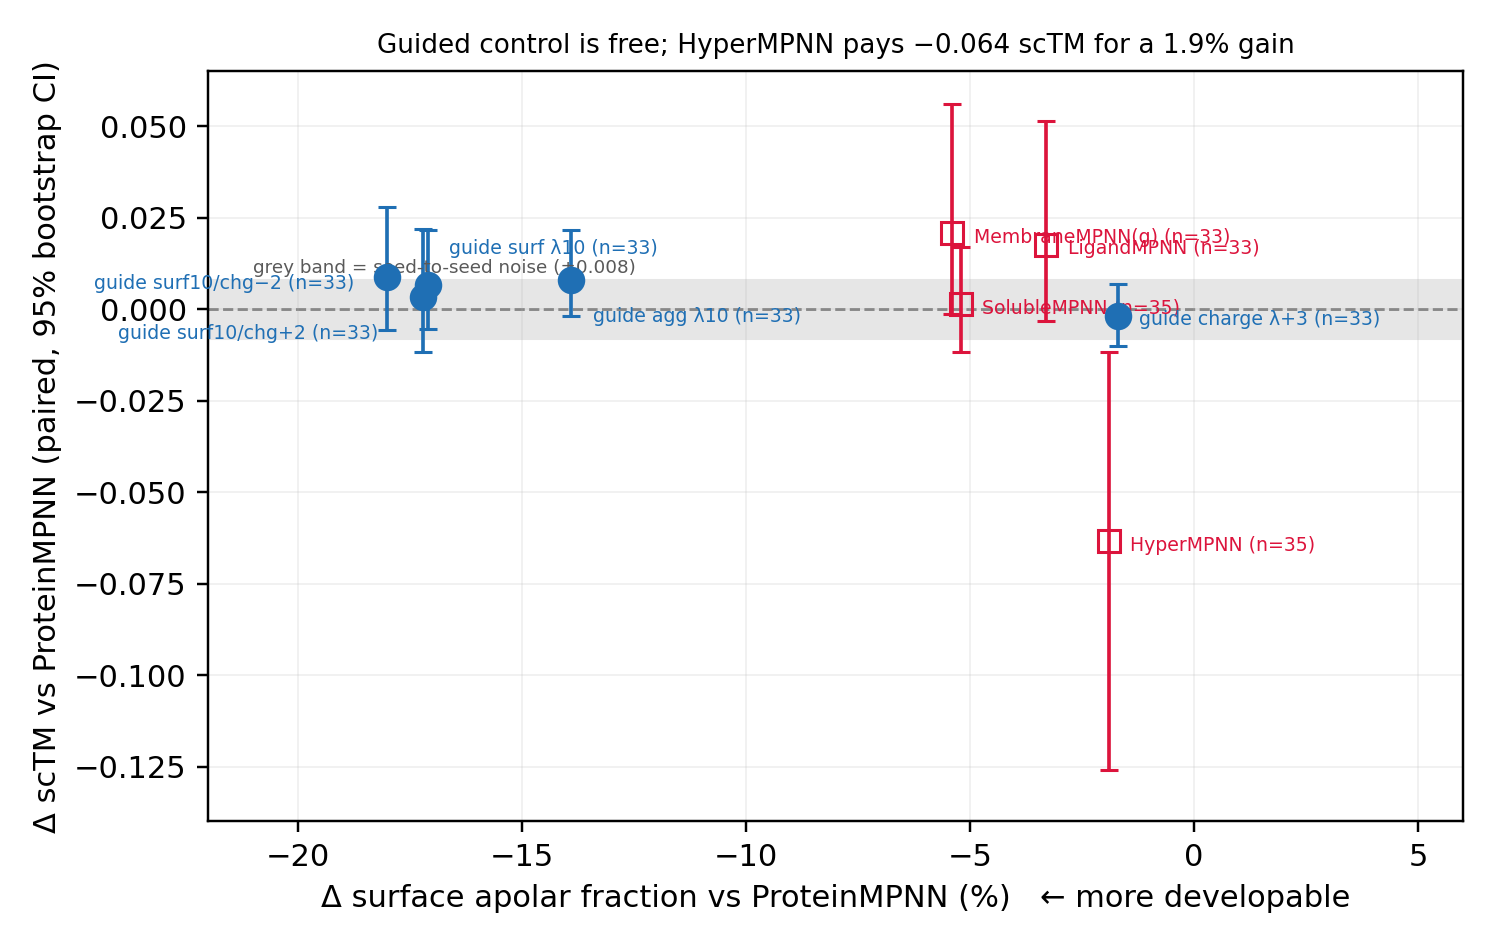
\includegraphics[width=0.62\linewidth]{figs/fig2_property_vs_sctm.png}
  \caption{Paired $\Delta$scTM versus $\Delta$ surface hydrophobicity. Grey
  band: reproducible seed-to-seed noise ($\pm 0.008$). All arms sit on the
  zero-cost line; guided arms (blue) move three times further left than
  published models (red).}
  \label{fig:property-vs-sctm}
\end{figure*}

\subsection*{4.1b Diversity is the real axis, and guidance moves the whole curve}
\label{sec:diversity-temperature}

Table~\ref{tab:main} sits at one temperature. Re-running the surface-guided arm
at $T = 0.3$ (33 backbones, 8 designs per cell, 264 folds;
Table~\ref{tab:temperature}) raises diversity from 0.277 to \textbf{0.390} ---
the same direction ProteinMPNN moves with temperature --- and simultaneously lets
guidance reach \textbf{$\bm{-70}$\% surface apolar and $\bm{-59}$\%
aggregation}. The paired cost of moving from $T{=}0.1$ to $T{=}0.3$ inside the
arm is $\Delta$scTM = $-0.0114$ (95\% CI $[-0.0228, +0.0016]$).

That is a genuine quality-diversity trade \textbf{within} the arm, and it makes
the comparison unambiguous: at $T{=}0.3$ the guided design set has
\textbf{higher diversity than the unguided baseline and higher scTM at once}
(0.390 and 0.8608 against 0.278 and 0.8434). For a model family where diversity
is a control variable rather than a nuisance, this is why we report the
(diversity, scTM, property) surface instead of a single operating point.

\subsection{Two properties, independently controlled}
\label{sec:control-plane}

On a 7-backbone pilot ($3\times3$ grid of surface
$\lambda \in \{0,5,10\}$ $\times$ charge $\lambda \in \{-2,0,+2\}$, 432 designs,
432 folds):

The full $3\times3$ grid of achieved (surface apolar, net charge) pairs is in
Table~\ref{tab:control-plane}; scTM across the whole plane stays in
0.9229--0.9348. Rows are nearly horizontal and columns nearly vertical: the two
axes are close to orthogonal. Table~\ref{tab:main} reproduces this
(surf10/charge$-2$ vs surf10/charge$+2$: surface 0.250 vs 0.258, charge $+12.83$
vs $-8.70$).

\setcounter{figure}{0}
\begin{figure*}[htbp]
  \centering
  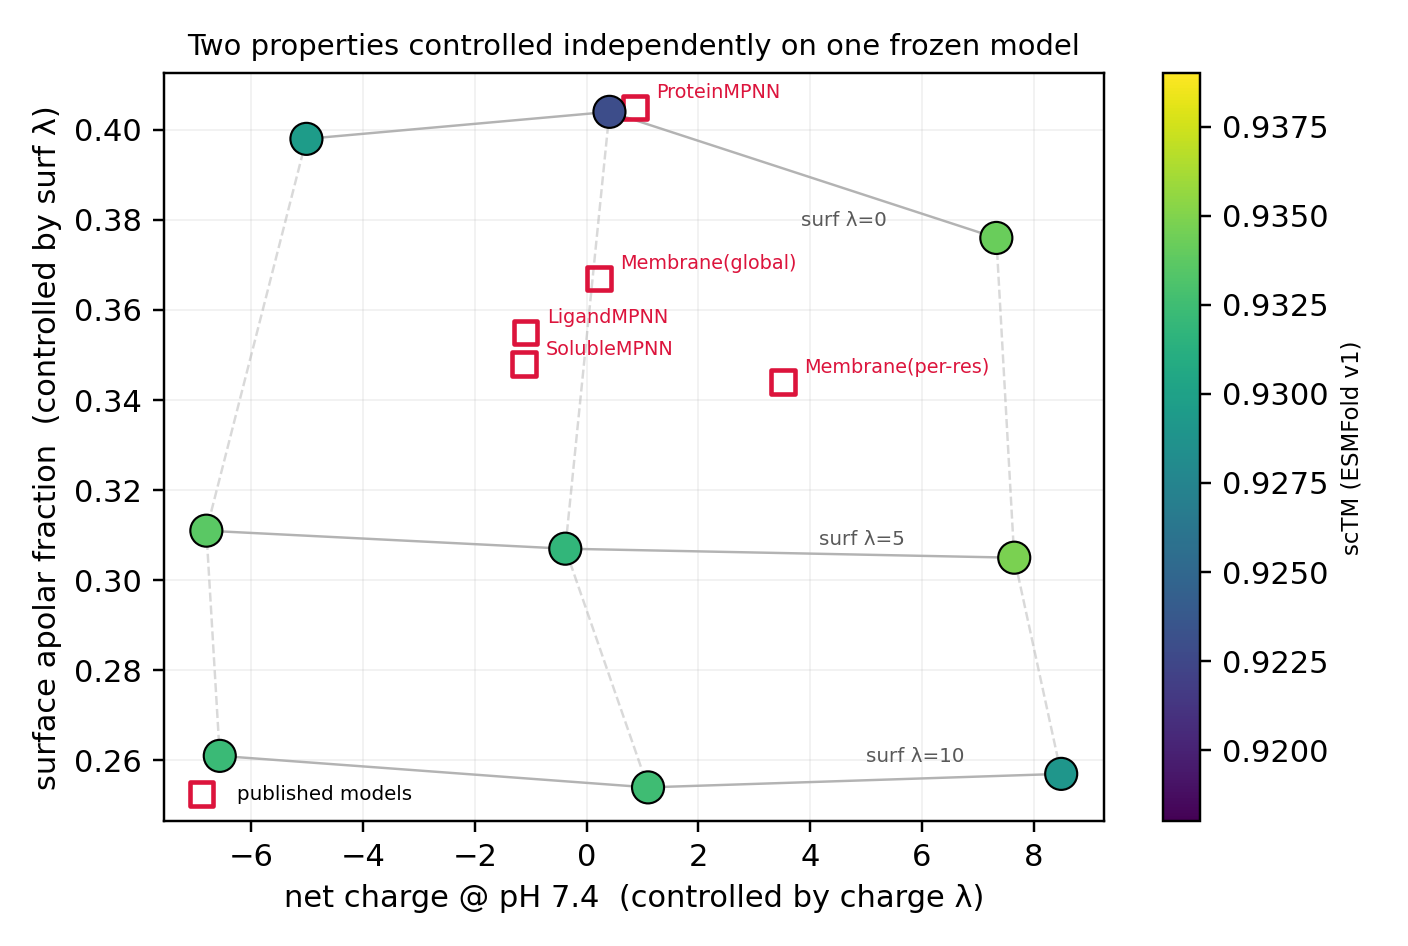
\includegraphics[width=0.62\linewidth]{figs/fig1_control_plane.png}
  \caption{The $3\times3$ control plane (filled circles, coloured by scTM)
  versus published models (open red squares), each of which is a single point.}
  \label{fig:control-plane}
\end{figure*}

\subsection{Controllability slope and leakage}
\label{sec:slope-leakage}

The slope \emph{k} is measured on the full benchmark, not a pilot. We swept the
surface objective over $\lambda \in \{2, 5, 10, 20\}$ with 16 designs per cell on
all 35 backbones (560 designs per $\lambda$, 2,240 designs, all folded):

\begin{table*}[htbp]
  \centering
  \footnotesize
  \setlength{\tabcolsep}{2pt}
  \begin{tabular}{@{}lrrrrr@{}}
    \toprule
    $\lambda$ & surface apolar & aggregation 5-mer & net charge & scTM & $\Delta$scTM vs ProteinMPNN [95\% CI] \\
    \midrule
    2 & 0.368 & 0.171 & $+2.08$ & 0.8472 & $+0.0028$ $[-0.0006, +0.0067]$ \\
    5 & 0.308 & 0.136 & $+1.60$ & 0.8472 & $+0.0028$ $[-0.0054, +0.0123]$ \\
    10 & 0.253 & 0.114 & $+1.52$ & 0.8507 & $+0.0062$ $[-0.0051, +0.0207]$ \\
    20 & $\bm{0.178}$ & 0.094 & $+1.74$ & 0.8471 & $+0.0027$ $[-0.0133, +0.0218]$ \\
    \bottomrule
  \end{tabular}
  \caption{Surface-objective sweep on the full benchmark ($\lambda \in \{2,5,10,20\}$,
  16 designs per cell, 35 backbones).}
  \label{tab:lambda-sweep}
\end{table*}

Fitting a line per backbone (OLS over the four $\lambda$ values) and averaging
over backbones gives \textbf{$k_{\mathrm{surface}} = \bm{-0.01005}$
surface-apolar fraction per $\lambda$ unit}, 95\% bootstrap CI
$[-0.01113, -0.00905]$, with mean per-backbone $R^2 = \bm{0.940}$ and a usable
fit on 35 of 35 backbones. One $\lambda$ unit therefore buys about one
percentage point of surface apolarity, and the relation is linear over a
factor-of-ten range of control strength: $\lambda{=}20$ reaches 0.178, a
\textbf{58.6\% relative reduction} from the ProteinMPNN baseline of 0.430.

The corresponding slope for foldability is
\textbf{$k_{\mathrm{scTM}} = \bm{+0.00001}$ scTM per $\lambda$ unit} (CI
$[-0.00072, +0.00083]$, $p = 0.98$). Foldability is flat across the entire
sweep, and no arm's interval at any $\lambda$ excludes zero. This is the
quantitative form of ``control is free'': not that one operating point happens
to be cheap, but that the cost stays flat while the targeted property moves by a
factor of two.

\textbf{The exposure mask is load-bearing.} A control experiment at
$\lambda{=}20$ applies the same apolar penalty to \emph{all} positions instead
of only the less-buried half. It controls the target somewhat better (surface
0.159 vs 0.178, paired $\Delta = -0.019$; aggregation 0.028 vs 0.094) but pays
for it: \textbf{$\Delta$scTM = $\bm{-0.0325}$} against the masked arm (95\% CI
$[-0.0748, -0.0019]$, $p = 0.028$), and it leaks composition (net charge +3.28
vs +1.74, pI 8.29 vs 7.96). The position-specific part of the reward is
therefore what keeps control from damaging foldability, and a benchmark that
only measured the targeted property would have scored the worse method as
better.

\textbf{Leakage is a property of the reward's weight vector, not of the model.}
Kyte--Doolittle assigns negative weights to K and R, so optimising GRAVY
necessarily loads positive charge: at $\lambda{=}4$ on the pilot set, GRAVY is
$-1.63$ with net charge $+9.6$ and pI 9.8, while scTM stays at 0.926. The
aggregation reward, whose weight vector is nearly orthogonal to charge, leaks
0.0 units. Surface targeting leaks into aggregation monotonically (0.171 $\to$
0.094 across the sweep) because the two penalties share the apolar residue set,
but leaves charge and pI near the baseline.

\setcounter{figure}{2}
\begin{figure*}[htbp]
  \centering
  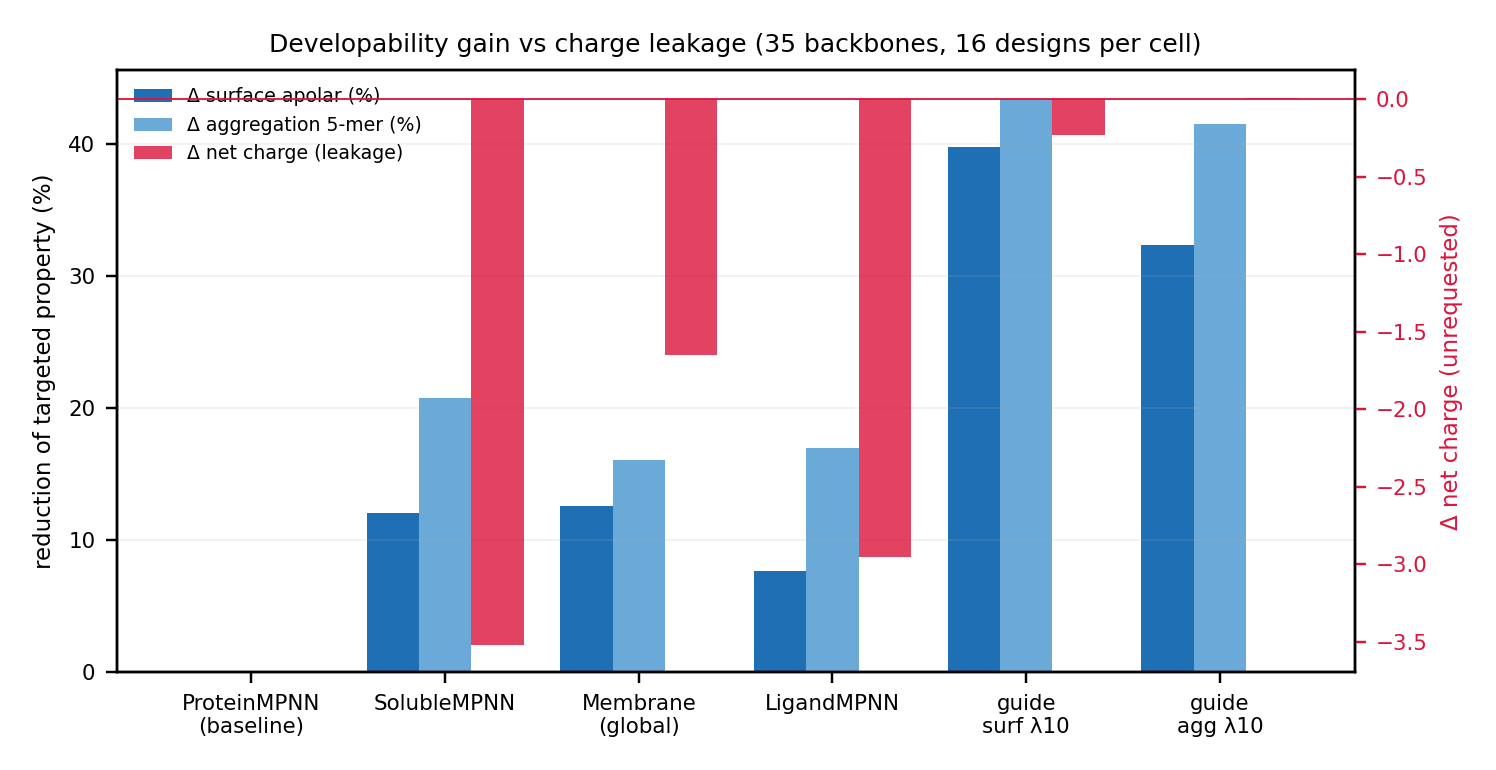
\includegraphics[width=0.62\linewidth]{figs/fig3_leakage.png}
  \caption{Targeted gain versus charge leakage for the four published arms plus the
  two surface/aggregation guided arms. Published models leak 1.7 to 3.5 charge
  units for a 4 to 13\% surface gain; the aggregation arm leaks 0.0 for a 42\%
  aggregation gain.}
  \label{fig:leakage}
\end{figure*}

\subsection{Oracle agreement: the conclusion holds, the ranking does not}
\label{sec:oracle}

We refolded 9 arms $\times$ 6 backbones $\times$ 2 designs (108 requested, 104 folded) with
\textbf{Protenix-2}~\cite{protenix} in single-sequence mode
(\texttt{--use\_msa False}), an architecture unrelated to
ESMFold~\cite{esmfold}.

Per-arm values for both oracles are in Table~\ref{tab:oracle}. Three observations:
Three observations:
\begin{enumerate}
\item \textbf{Absolute scale differs by 0.15} (ESMFold $\approx$0.93,
  single-sequence Protenix $\approx$0.72--0.81), so scTM is not comparable
  across oracles.
\item \textbf{Arm ranking is essentially unrelated}: Spearman across the 9 arms
  = $\bm{-0.18}$ ($p = 0.64$) --- the two oracles do not rank the arms
  consistently on this subset.
\item \textbf{The claim survives}: under Protenix \emph{every} arm beats
  vanilla ($+0.01$ to $+0.08$), with the two guidance arms on top; under
  ESMFold every arm is within $\pm 0.008$ of vanilla. ``Control does not cost
  foldability'' is oracle-robust even though ``which arm is best'' is not.
\end{enumerate}

Per-design correlation between the two oracles is \textbf{negative}
($n = 98$, Pearson $-0.45$, Spearman $-0.48$): ESMFold's scores are compressed
at the 0.92--0.94 ceiling, so its residual ordering is noise dominated.

\emph{Caveat.} The Protenix run is single-sequence (no MSA), a deliberately
cheap and degraded usage; it is used only to test direction, not to rank.

\subsection*{4.5 Per-backbone heterogeneity: arm means hide bimodal failure}
\label{sec:heterogeneity}

Averaging over 35 backbones is a lossy summary, and the loss matters here.

(Per-arm medians, means and worst-case collapses are in
Table~\ref{tab:heterogeneity}; the paragraphs below use them.)


HyperMPNN is the clearest case. On the \textbf{median backbone it differs from
ProteinMPNN by $\bm{-0.005}$}, and 26 of 35 backbones sit within $\pm 0.05$. But
three backbones collapse completely: 1SRL 0.220 vs 0.773, 1TIT 0.230 vs 0.862,
3PGK 0.164 vs 0.756. The mean $-0.064$ is therefore not ``a small uniform loss'';
it is \textbf{no change on most backbones plus catastrophic failure on 3 of 35},
and removing those three collapses brings the mean to $-0.014$. These are not
degenerate samples: all sixteen designs per cell are unique and their composition
entropy (3.3--4.0 bits) is indistinguishable from ProteinMPNN on the same
backbones, so the collapse is a property of the thermophile-trained prior on
these folds, not a sampling artefact.

Two consequences for benchmarking. First, \textbf{a per-arm mean is the wrong
summary statistic} for a model family where failure is bimodal; a benchmark
should report the per-backbone tail, which is why we release the full
$35 \times 10$ matrix (\texttt{results/b30\_designs.tsv}) instead of only the
aggregate. Second, \textbf{half of this benchmark has no discriminating power}:
13 of 35 backbones score above 0.92 for every arm with an arm-to-arm spread of
0.01--0.03, so any conclusion about arm differences comes from the roughly 15
backbones below 0.92.

The guided arms are the flattest: their median per-backbone change is
$\leq 0.002$ and their worst case is 0.18, an order of magnitude smaller than
the retrained or conditioned models. Whatever the guidance does, it does it
evenly.

\section{Discussion}
\label{sec:discussion}

\paragraph{Why is control nearly free?}
The properties are linear in composition, so guidance only re-weights first
moments at each position; it does not move the backbone-conditioned
high-density region. Consistent with this, the property-quality coupling we
measure \emph{between designs} is positive (GRAVY vs scTM $+0.61$, aggregation
vs scTM $+0.56$) but the range we move ($\Delta$GRAVY $\approx 0.4$) is small
relative to between-design dispersion, so no second-order collapse is
triggered.

\paragraph{When does it stop being free?}
Two observed boundaries: (i) pushing a property that is strongly coupled to
quality (GRAVY at $\lambda{=}4$ already lowers scTM to 0.9257, and
$\lambda{=}8$ yields unfolded sequences); (ii) pushing a property whose weight
vector is correlated with another (GRAVY $\to +20$ charge). Controllability is
therefore not a property of a model but of the (objective $\times$ weight
vector) pair.

\paragraph{Implications.}
For weakly coupled properties (surface hydrophobicity, net charge) retraining
is unnecessary: the closed-form tilt is larger in effect, reversible, and
cheaper. For strongly coupled objectives (stability, expression) a prior shift
or RL is still required. In both cases acceptance must report the properties
that were \emph{not} requested.

\section{Limitations}
\label{sec:limitations}

\begin{enumerate}
\item \textbf{Scope of properties}: only composition-linear objectives are
  covered, so the closed-form guidance applies; aggregation is approximated by a
  windowed exposure proxy, not a learned predictor. Guidance through a learned
  predictor (ProteinGuide's TAG) or through any non-linear objective is not
  tested here, and the paper should not be read as evidence about that class of
  methods.
\item \textbf{Scope of structures}: 35 monomers, all soluble and experimental;
  no membrane proteins, complexes or de novo backbones.
  Only one sampling temperature (0.1) is used for the main table.
\item \textbf{Oracles}: ESMFold v1 is the primary oracle and single-sequence
  Protenix-2 the check; both are weaker than the ESMFold2/Boltz-2 setting used
  by recent design papers, and feature-wise they disagree.
\item \textbf{Power}: 16 designs per (arm, backbone) and a $\pm 0.008$
  seed-to-seed floor; effects below that are unresolved. Only ProteinMPNN was
  replicated across seeds, and the temperature ablation in \S4.1b still uses the
  8-design run.
\item \textbf{No wet lab}: every property is a computational proxy; published
  correlations between sequence-side solubility predictors and measured yield
  are weak ($r \leq 0.32$).
\item \textbf{Backbone composition}: the 35 backbones skew small (19 of 35 under
  100 residues) and include 5 NMR entries, so absolute scTM values are
  optimistic for the 150--300 residue regime that real campaigns target. The
  paired design of every comparison removes most of this bias from arm-to-arm
  differences, but not from the absolute numbers.
\item \textbf{One alignment artefact}: for backbone 1TEN the ProteinMPNN-family
  arms emit 90 residues while chain A of the reference file has 89 C$\alpha$
  atoms (LigandMPNN emits 89), so those four arms are scored on a shifted
  alignment and collapse to $\sim$0.44 there while the LigandMPNN arms score
  $\sim$0.94 on the same backbone. The artefact is identical in the 8- and
  16-design runs, so it is not a regression, but it inflates the two LigandMPNN
  arms' paired means by roughly $+0.015$. Excluding 1TEN, MembraneMPNN's estimate
  falls from $+0.021$ to $+0.006$ (CI $[-0.003, +0.018]$) and LigandMPNN's from
  $+0.018$ to $+0.003$, while no other arm moves; we therefore do not claim a
  membrane or ligand scTM gain from this benchmark.
\end{enumerate}


% Page-count marker for the main text: the last body page is recorded in
% main.aux as the page of this label (References and appendices follow).
\label{endofbody}

\bibliographystyle{plainnat}
\bibliography{refs}

\section*{Appendix A --- Property definitions}
\label{app:properties}

\begin{itemize}
\item \textbf{Net charge @ pH 7.4}: Henderson--Hasselbalch over D/E/C/Y/H/K/R
  with standard pKa, plus termini, divided by length.
\item \textbf{pI}: bisection root of the charge curve.
\item \textbf{GRAVY}: Kyte--Doolittle mean.
\item \textbf{Surface apolar fraction}: exposure from the \emph{input}
  backbone (CA neighbours within 10\,\AA; the less-buried half of residues
  counts as exposed); fraction of \{G,P,A,V,I,L,M,F,W,Y\} at exposed sites.
  \emph{Validation}: against a Shrake--Rupley SASA computed on N/CA/C/O with a
  1.4\,\AA{} probe, the CA-burial exposure
  agrees on 65--76\% of residues (chance 50\%) and Spearman-correlates with
  real SASA at $\rho = -0.38$ to $-0.59$ on the
  six backbones tested. The proxy is therefore informative but coarse, and
  absolute surface numbers should not be
  compared with SASA-based hydrophobicity scores such as SAP.
\item \textbf{Aggregation 5-mer fraction}: fraction of 5-residue windows that
  are $\geq$80\% apolar.
\item \textbf{Recovery}: identity to the native sequence at aligned positions.
\item \textbf{Diversity}: mean pairwise Hamming distance over the designs of one
  (arm, backbone) cell (16 in the main run).
\end{itemize}

\section*{Appendix B --- Additional tables}
\label{app:additional-tables}

% Tables moved out of the body in the v3 revision; they are numbered B.1--B.3
% (the body tables are 1--6). The body forward-references them via \ref.
\renewcommand{\thetable}{B.\arabic{table}}
\setcounter{table}{0}

\begin{table}[H]
  \centering
  \small
  \caption{\textbf{Composition of the 35-backbone set.}}
  \label{tab:backbones}
  \begin{tabular}{@{}ll@{}}
    \toprule
    property & value \\
    \midrule
    backbones & 35 \\
    length & median 91, mean 133, range 56--415 \\
    length bins & $<$100 aa: 19 $\cdot$ 100--200: 9 $\cdot$ 200--300: 4 $\cdot$ 300--500: 3 \\
    experimental method & X-ray 30, NMR 5 \\
    X-ray resolution & median 1.80\,\AA, range 1.00--2.70\,\AA \\
    \bottomrule
  \end{tabular}
\end{table}

\begin{table}[H]
  \centering
  \small
  \caption{\textbf{The $3\times3$ control plane (7 backbones, 432 designs).}
  Cells are surface apolar fraction / net charge; scTM is 0.9229--0.9348 across
  the plane. Rows move surface apolarity and leave charge roughly unchanged;
  columns do the converse.}
  \label{tab:control-plane}
  \begin{tabular}{@{}lrrr@{}}
    \toprule
    surf $\lambda$ \textbackslash{} charge $\lambda$ & $-2$ & 0 & $+2$ \\
    \midrule
    0 & 0.376 / $+7.33$ & 0.404 / $+0.41$ & 0.398 / $-5.01$ \\
    5 & 0.305 / $+7.65$ & 0.307 / $-0.38$ & 0.311 / $-6.80$ \\
    10 & 0.257 / $+8.49$ & 0.254 / $+1.10$ & 0.261 / $-6.56$ \\
    \bottomrule
  \end{tabular}
\end{table}

\begin{table}[H]
  \centering
  \small
  \setlength{\tabcolsep}{5pt}
  \caption{\textbf{Oracle comparison on the same 104 folded structures.}}
  \label{tab:oracle}
  \begin{tabular}{@{}lrrr@{}}
    \toprule
    Arm & Protenix-2 scTM & $\Delta$ vs vanilla & ESMFold $\Delta$ (same subset) \\
    \midrule
    vanilla & 0.7238 & --- & --- \\
    SolubleMPNN & 0.7877 & $+0.0639$ & $-0.0044$ \\
    MembraneMPNN (global) & 0.7332 & $+0.0094$ & $-0.0078$ \\
    LigandMPNN & 0.7383 & $+0.0145$ & $-0.0027$ \\
    guide surf $\lambda$10 & $\bm{0.8050}$ & $\bm{+0.0812}$ & $-0.0039$ \\
    guide agg $\lambda$10 & 0.7936 & $+0.0698$ & $-0.0023$ \\
    guide charge $\lambda{+}3$ & 0.7775 & $+0.0537$ & $-0.0006$ \\
    guide surf10/charge$-2$ & 0.7797 & $+0.0559$ & $-0.0066$ \\
    guide surf10/charge$+2$ & 0.7747 & $+0.0509$ & $-0.0035$ \\
    \bottomrule
  \end{tabular}
\end{table}
\begin{table}[H]
  \centering
  \footnotesize
  \setlength{\tabcolsep}{3pt}
  \caption{\textbf{Temperature ablation of the surface-guided arm (33 backbones,
  8 designs per cell).} The $T{=}0.1$ rows are the 8-design reference run, not
  the 16-design main table.}
  \label{tab:temperature}
  \begin{tabular}{@{}lrrrrr@{}}
    \toprule
    arm & diversity & scTM & surface apolar & aggregation 5-mer & recovery \\
    \midrule
    ProteinMPNN ($T{=}0.1$, 8 designs) & 0.278 & 0.8434 & 0.438 & 0.217 & 0.439 \\
    guide surf $\lambda$10 ($T{=}0.1$) & 0.277 & 0.8721 & 0.259 & 0.122 & 0.448 \\
    \textbf{guide surf $\lambda$10 ($T{=}0.3$)} & \textbf{0.390} & \textbf{0.8608} & \textbf{0.133} & \textbf{0.089} & 0.411 \\
    \bottomrule
  \end{tabular}
\end{table}

\begin{table}[H]
  \centering
  \footnotesize
  \setlength{\tabcolsep}{2pt}
  \caption{\textbf{Per-backbone heterogeneity of the paired $\Delta$scTM.}}
  \label{tab:heterogeneity}
  \begin{tabular}{@{}lrrrr@{}}
    \toprule
    arm & \shortstack[r]{median per-backbone\\$\Delta$scTM} & \shortstack[r]{mean\\$\Delta$scTM} & \shortstack[r]{mean excluding\\collapses} & \shortstack[r]{max per-backbone\\collapse} \\
    \midrule
    SolubleMPNN & $-0.001$ & $+0.0013$ & --- & 0.15 \\
    \textbf{HyperMPNN} & $\bm{-0.005}$ & $\bm{-0.0635}$ & $\bm{-0.0140}$ & $\bm{0.63}$ \\
    MembraneMPNN (global) & $-0.001$ & $+0.0207$ & --- & 0.49 \\
    LigandMPNN & $+0.002$ & $+0.0176$ & --- & 0.50 \\
    guide surf $\lambda$10 & $+0.001$ & $+0.0066$ & --- & 0.18 \\
    guide agg $\lambda$10 & $+0.001$ & $+0.0081$ & --- & 0.16 \\
    guide charge $\lambda{+}3$ & $-0.001$ & $-0.0019$ & --- & 0.09 \\
    \bottomrule
  \end{tabular}
\end{table}

\section*{Appendix C --- Reproducibility and data availability}
\label{app:reproducibility}

\begin{itemize}
\item Code: \texttt{prep\_targets.py}, \texttt{guided\_run.py},
  \texttt{bench30\_grid.py}, \texttt{agg\_grid.py}, \texttt{dev\_fold.py},
  \texttt{analyze\_bench30.py}, \texttt{px\_batch.py}, \texttt{px\_eval.py}.
\item Data: \texttt{runs/bench30\_p16/\{arm\}/\{backbone\}/seqs/*.fa} (5,936
  designs) and \texttt{results/p16/AGGREGATE\_P16.md} (the 16-design aggregate
  that every \S4.1 number comes from), plus the 8-design predecessor
  \texttt{runs/bench30/\{arm\}/\{backbone\}/seqs/*.fa} (2,688 designs) used for
  the \S4.1b ablation, \texttt{results/b30\_designs.tsv} (the full per-design
  matrix: arm $\times$ backbone $\times$ design with properties, recovery and
  diversity, the source of every per-backbone number in \S4.5),
  \texttt{runs/px/px\_scTM.tsv} (Protenix fold-ins), plus
  \texttt{results/AGGREGATE.md} (deduplicated aggregate with paired bootstrap
  and Holm columns).
\item Backbone list: \texttt{data/targets30.txt}.
\item Environment: Python 3.11, torch 2.2.2, fair-esm ESMFold v1 with a
  vendored openfold (three patches documented in the repository), Protenix-2 in
  its own environment with \texttt{--use\_msa False}.
\item Dataset documentation: \texttt{DATASHEET.md}; artifact entry point:
  \texttt{README.md} (setup, reproduction order, known pitfalls); runtime pins:
  \texttt{requirements.txt}; licence: \texttt{LICENSE} (code MIT, text and
  figures CC BY 4.0).
\item Evaluation harness used for the second oracle: Protenix-2 with
  \texttt{--use\_msa False}; per-sequence fold-ins in
  \texttt{results/px\_scTM.tsv}.
\item Figures: \texttt{figs/fig1\_control\_plane.png},
  \texttt{figs/fig2\_property\_vs\_sctm.png},
  \texttt{figs/fig3\_leakage.png}.
\end{itemize}

% NeurIPS 2026 Paper Checklist. Copied from the official formatted template
% (checklist.tex in the NeurIPS 2026 formatting zip); the instruction block has
% been deleted as the official instructions require. All answers are left as
% \answerTODO / \justificationTODO placeholders for the authors to fill in.

\section*{NeurIPS Paper Checklist}

\begin{enumerate}

\item {\bf Claims}
    \item[] Question: Do the main claims made in the abstract and introduction accurately reflect the paper's contributions and scope?
    \item[] Answer: \answerYes{}
    \item[] Justification: The abstract and \S1 state the five evaluation-practice findings and the three measurements (controllability slope, leakage, per-backbone tail) with the numbers that support them, and \S6 enumerates the scope limits (single regime, composition-linear objectives, no wet lab). The claims are measurements on the released design matrix rather than extrapolations.
    \item[] Guidelines:
    \begin{itemize}
        \item The answer \answerNA{} means that the abstract and introduction do not include the claims made in the paper.
        \item The abstract and/or introduction should clearly state the claims made, including the contributions made in the paper and important assumptions and limitations. A \answerNo{} or \answerNA{} answer to this question will not be perceived well by the reviewers. 
        \item The claims made should match theoretical and experimental results, and reflect how much the results can be expected to generalize to other settings. 
        \item It is fine to include aspirational goals as motivation as long as it is clear that these goals are not attained by the paper. 
    \end{itemize}

\item {\bf Limitations}
    \item[] Question: Does the paper discuss the limitations of the work performed by the authors?
    \item[] Answer: \answerYes{}
    \item[] Justification: \S6 Limitations lists seven items, including the single scenario, the small-backbone skew, the coarse property proxies, the single temperature, the absence of wet-lab validation, the oracle choice, and a documented 1TEN alignment artefact with its exclusion sensitivity analysis.
    \item[] Guidelines:
    \begin{itemize}
        \item The answer \answerNA{} means that the paper has no limitation while the answer \answerNo{} means that the paper has limitations, but those are not discussed in the paper. 
        \item The authors are encouraged to create a separate ``Limitations'' section in their paper.
        \item The paper should point out any strong assumptions and how robust the results are to violations of these assumptions (e.g., independence assumptions, noiseless settings, model well-specification, asymptotic approximations only holding locally). The authors should reflect on how these assumptions might be violated in practice and what the implications would be.
        \item The authors should reflect on the scope of the claims made, e.g., if the approach was only tested on a few datasets or with a few runs. In general, empirical results often depend on implicit assumptions, which should be articulated.
        \item The authors should reflect on the factors that influence the performance of the approach. For example, a facial recognition algorithm may perform poorly when image resolution is low or images are taken in low lighting. Or a speech-to-text system might not be used reliably to provide closed captions for online lectures because it fails to handle technical jargon.
        \item The authors should discuss the computational efficiency of the proposed algorithms and how they scale with dataset size.
        \item If applicable, the authors should discuss possible limitations of their approach to address problems of privacy and fairness.
        \item While the authors might fear that complete honesty about limitations might be used by reviewers as grounds for rejection, a worse outcome might be that reviewers discover limitations that aren't acknowledged in the paper. The authors should use their best judgment and recognize that individual actions in favor of transparency play an important role in developing norms that preserve the integrity of the community. Reviewers will be specifically instructed to not penalize honesty concerning limitations.
    \end{itemize}

\item {\bf Theory assumptions and proofs}
    \item[] Question: For each theoretical result, does the paper provide the full set of assumptions and a complete (and correct) proof?
    \item[] Answer: \answerNA{}
    \item[] Justification: The paper contains no theorems. The closed form in \S3.3 is a one-line algebraic consequence of the AO-ARM factorisation and is derived in place rather than stated as a theoretical result.
    \item[] Guidelines:
    \begin{itemize}
        \item The answer \answerNA{} means that the paper does not include theoretical results. 
        \item All the theorems, formulas, and proofs in the paper should be numbered and cross-referenced.
        \item All assumptions should be clearly stated or referenced in the statement of any theorems.
        \item The proofs can either appear in the main paper or the supplemental material, but if they appear in the supplemental material, the authors are encouraged to provide a short proof sketch to provide intuition. 
        \item Inversely, any informal proof provided in the core of the paper should be complemented by formal proofs provided in appendix or supplemental material.
        \item Theorems and Lemmas that the proof relies upon should be properly referenced. 
    \end{itemize}

    \item {\bf Experimental result reproducibility}
    \item[] Question: Does the paper fully disclose all the information needed to reproduce the main experimental results of the paper to the extent that it affects the main claims and/or conclusions of the paper (regardless of whether the code and data are provided or not)?
    \item[] Answer: \answerYes{}
    \item[] Justification: \S3 gives the backbone list, the 11 arms with their exact checkpoints and command-line recipes, the sampling temperature and seeds, the ESMFold/Protenix settings, and the aggregation and bootstrap procedure; Appendix C lists every code and data file needed to regenerate the tables.
    \item[] Guidelines:
    \begin{itemize}
        \item The answer \answerNA{} means that the paper does not include experiments.
        \item If the paper includes experiments, a \answerNo{} answer to this question will not be perceived well by the reviewers: Making the paper reproducible is important, regardless of whether the code and data are provided or not.
        \item If the contribution is a dataset and\slash or model, the authors should describe the steps taken to make their results reproducible or verifiable. 
        \item Depending on the contribution, reproducibility can be accomplished in various ways. For example, if the contribution is a novel architecture, describing the architecture fully might suffice, or if the contribution is a specific model and empirical evaluation, it may be necessary to either make it possible for others to replicate the model with the same dataset, or provide access to the model. In general. releasing code and data is often one good way to accomplish this, but reproducibility can also be provided via detailed instructions for how to replicate the results, access to a hosted model (e.g., in the case of a large language model), releasing of a model checkpoint, or other means that are appropriate to the research performed.
        \item While NeurIPS does not require releasing code, the conference does require all submissions to provide some reasonable avenue for reproducibility, which may depend on the nature of the contribution. For example
        \begin{enumerate}
            \item If the contribution is primarily a new algorithm, the paper should make it clear how to reproduce that algorithm.
            \item If the contribution is primarily a new model architecture, the paper should describe the architecture clearly and fully.
            \item If the contribution is a new model (e.g., a large language model), then there should either be a way to access this model for reproducing the results or a way to reproduce the model (e.g., with an open-source dataset or instructions for how to construct the dataset).
            \item We recognize that reproducibility may be tricky in some cases, in which case authors are welcome to describe the particular way they provide for reproducibility. In the case of closed-source models, it may be that access to the model is limited in some way (e.g., to registered users), but it should be possible for other researchers to have some path to reproducing or verifying the results.
        \end{enumerate}
    \end{itemize}


\item {\bf Open access to data and code}
    \item[] Question: Does the paper provide open access to the data and code, with sufficient instructions to faithfully reproduce the main experimental results, as described in supplemental material?
    \item[] Answer: \answerYes{}
    \item[] Justification: Code, the per-design matrix, both aggregates, the artifact README with the reproduction order, the runtime pins and the licence are released with the submission; the PDB accessions needed to rebuild the backbone set are listed so the inputs can be re-fetched.
    \item[] Guidelines:
    \begin{itemize}
        \item The answer \answerNA{} means that paper does not include experiments requiring code.
        \item Please see the NeurIPS code and data submission guidelines (\url{https://neurips.cc/public/guides/CodeSubmissionPolicy}) for more details.
        \item While we encourage the release of code and data, we understand that this might not be possible, so \answerNo{} is an acceptable answer. Papers cannot be rejected simply for not including code, unless this is central to the contribution (e.g., for a new open-source benchmark).
        \item The instructions should contain the exact command and environment needed to run to reproduce the results. See the NeurIPS code and data submission guidelines (\url{https://neurips.cc/public/guides/CodeSubmissionPolicy}) for more details.
        \item The authors should provide instructions on data access and preparation, including how to access the raw data, preprocessed data, intermediate data, and generated data, etc.
        \item The authors should provide scripts to reproduce all experimental results for the new proposed method and baselines. If only a subset of experiments are reproducible, they should state which ones are omitted from the script and why.
        \item At submission time, to preserve anonymity, the authors should release anonymized versions (if applicable).
        \item Providing as much information as possible in supplemental material (appended to the paper) is recommended, but including URLs to data and code is permitted.
    \end{itemize}


\item {\bf Experimental setting/details}
    \item[] Question: Does the paper specify all the training and test details (e.g., data splits, hyperparameters, how they were chosen, type of optimizer) necessary to understand the results?
    \item[] Answer: \answerYes{}
    \item[] Justification: No model is trained in this paper, so there are no optimizer or split choices. All inference details are given in \S3.2 and \S3.5: checkpoints, temperatures (0.1 for the main table, 0.3 for the ablation), seeds (0 and 1), 16 designs per cell, and the exposure/charge definitions in Appendix A.
    \item[] Guidelines:
    \begin{itemize}
        \item The answer \answerNA{} means that the paper does not include experiments.
        \item The experimental setting should be presented in the core of the paper to a level of detail that is necessary to appreciate the results and make sense of them.
        \item The full details can be provided either with the code, in appendix, or as supplemental material.
    \end{itemize}

\item {\bf Experiment statistical significance}
    \item[] Question: Does the paper report error bars suitably and correctly defined or other appropriate information about the statistical significance of the experiments?
    \item[] Answer: \answerYes{}
    \item[] Justification: Every arm comparison is paired over backbones with a 10,000-sample bootstrap, reported with 95\% percentile intervals, raw and Holm-adjusted p-values, and a stated minimum detectable effect (0.0147 scTM after correction). The seed-to-seed replicate gives the measurement floor (0.008 scTM).
    \item[] Guidelines:
    \begin{itemize}
        \item The answer \answerNA{} means that the paper does not include experiments.
        \item The authors should answer \answerYes{} if the results are accompanied by error bars, confidence intervals, or statistical significance tests, at least for the experiments that support the main claims of the paper.
        \item The factors of variability that the error bars are capturing should be clearly stated (for example, train/test split, initialization, random drawing of some parameter, or overall run with given experimental conditions).
        \item The method for calculating the error bars should be explained (closed form formula, call to a library function, bootstrap, etc.)
        \item The assumptions made should be given (e.g., Normally distributed errors).
        \item It should be clear whether the error bar is the standard deviation or the standard error of the mean.
        \item It is OK to report 1-sigma error bars, but one should state it. The authors should preferably report a 2-sigma error bar than state that they have a 96\% CI, if the hypothesis of Normality of errors is not verified.
        \item For asymmetric distributions, the authors should be careful not to show in tables or figures symmetric error bars that would yield results that are out of range (e.g., negative error rates).
        \item If error bars are reported in tables or plots, the authors should explain in the text how they were calculated and reference the corresponding figures or tables in the text.
    \end{itemize}

\item {\bf Experiments compute resources}
    \item[] Question: For each experiment, does the paper provide sufficient information on the computer resources (type of compute workers, memory, time of execution) needed to reproduce the experiments?
    \item[] Answer: \answerYes{}
    \item[] Justification: \S3.5 and Appendix C state the hardware (up to four RTX A6000 GPUs, never more than four concurrently), the wall-clock budget of the sweep, and that no training is involved; folding dominates the runtime.
    \item[] Guidelines:
    \begin{itemize}
        \item The answer \answerNA{} means that the paper does not include experiments.
        \item The paper should indicate the type of compute workers CPU or GPU, internal cluster, or cloud provider, including relevant memory and storage.
        \item The paper should provide the amount of compute required for each of the individual experimental runs as well as estimate the total compute. 
        \item The paper should disclose whether the full research project required more compute than the experiments reported in the paper (e.g., preliminary or failed experiments that didn't make it into the paper). 
    \end{itemize}
    
\item {\bf Code of ethics}
    \item[] Question: Does the research conducted in the paper conform, in every respect, with the NeurIPS Code of Ethics \url{https://neurips.cc/public/EthicsGuidelines}?
    \item[] Answer: \answerYes{}
    \item[] Justification: The work uses public PDB structures and released model weights, involves no human subjects, and reports failure modes of published methods rather than optimising a deployable design pipeline.
    \item[] Guidelines:
    \begin{itemize}
        \item The answer \answerNA{} means that the authors have not reviewed the NeurIPS Code of Ethics.
        \item If the authors answer \answerNo, they should explain the special circumstances that require a deviation from the Code of Ethics.
        \item The authors should make sure to preserve anonymity (e.g., if there is a special consideration due to laws or regulations in their jurisdiction).
    \end{itemize}


\item {\bf Broader impacts}
    \item[] Question: Does the paper discuss both potential positive societal impacts and negative societal impacts of the work performed?
    \item[] Answer: \answerNA{}
    \item[] Justification: The paper analyses evaluation practice for protein-design models; it releases no generative model and no design pipeline that could be misused, and \S5 discusses the practical implication for how such methods should be benchmarked rather than how to build better ones.
    \item[] Guidelines:
    \begin{itemize}
        \item The answer \answerNA{} means that there is no societal impact of the work performed.
        \item If the authors answer \answerNA{} or \answerNo, they should explain why their work has no societal impact or why the paper does not address societal impact.
        \item Examples of negative societal impacts include potential malicious or unintended uses (e.g., disinformation, generating fake profiles, surveillance), fairness considerations (e.g., deployment of technologies that could make decisions that unfairly impact specific groups), privacy considerations, and security considerations.
        \item The conference expects that many papers will be foundational research and not tied to particular applications, let alone deployments. However, if there is a direct path to any negative applications, the authors should point it out. For example, it is legitimate to point out that an improvement in the quality of generative models could be used to generate Deepfakes for disinformation. On the other hand, it is not needed to point out that a generic algorithm for optimizing neural networks could enable people to train models that generate Deepfakes faster.
        \item The authors should consider possible harms that could arise when the technology is being used as intended and functioning correctly, harms that could arise when the technology is being used as intended but gives incorrect results, and harms following from (intentional or unintentional) misuse of the technology.
        \item If there are negative societal impacts, the authors could also discuss possible mitigation strategies (e.g., gated release of models, providing defenses in addition to attacks, mechanisms for monitoring misuse, mechanisms to monitor how a system learns from feedback over time, improving the efficiency and accessibility of ML).
    \end{itemize}
    
\item {\bf Safeguards}
    \item[] Question: Does the paper describe safeguards that have been put in place for responsible release of data or models that have a high risk for misuse (e.g., pre-trained language models, image generators, or scraped datasets)?
    \item[] Answer: \answerNA{}
    \item[] Justification: No model, generator or scraped dataset with misuse risk is released. The released artifact is a measurement matrix and the code that produced it.
    \item[] Guidelines:
    \begin{itemize}
        \item The answer \answerNA{} means that the paper poses no such risks.
        \item Released models that have a high risk for misuse or dual-use should be released with necessary safeguards to allow for controlled use of the model, for example by requiring that users adhere to usage guidelines or restrictions to access the model or implementing safety filters. 
        \item Datasets that have been scraped from the Internet could pose safety risks. The authors should describe how they avoided releasing unsafe images.
        \item We recognize that providing effective safeguards is challenging, and many papers do not require this, but we encourage authors to take this into account and make a best faith effort.
    \end{itemize}

\item {\bf Licenses for existing assets}
    \item[] Question: Are the creators or original owners of assets (e.g., code, data, models), used in the paper, properly credited and are the license and terms of use explicitly mentioned and properly respected?
    \item[] Answer: \answerYes{}
    \item[] Justification: \S2 credits ProteinMPNN, SolubleMPNN, HyperMPNN, MembraneMPNN and LigandMPNN with their papers and repositories, and the released weights are used under their upstream licences; the artefact README records these terms and the PDB public-domain status.
    \item[] Guidelines:
    \begin{itemize}
        \item The answer \answerNA{} means that the paper does not use existing assets.
        \item The authors should cite the original paper that produced the code package or dataset.
        \item The authors should state which version of the asset is used and, if possible, include a URL.
        \item The name of the license (e.g., CC-BY 4.0) should be included for each asset.
        \item For scraped data from a particular source (e.g., website), the copyright and terms of service of that source should be provided.
        \item If assets are released, the license, copyright information, and terms of use in the package should be provided. For popular datasets, \url{paperswithcode.com/datasets} has curated licenses for some datasets. Their licensing guide can help determine the license of a dataset.
        \item For existing datasets that are re-packaged, both the original license and the license of the derived asset (if it has changed) should be provided.
        \item If this information is not available online, the authors are encouraged to reach out to the asset's creators.
    \end{itemize}

\item {\bf New assets}
    \item[] Question: Are new assets introduced in the paper well documented and is the documentation provided alongside the assets?
    \item[] Answer: \answerYes{}
    \item[] Justification: The new assets (the 35-backbone evaluation set with fixed accessions, the 5,936-design matrix, the two aggregates and the Croissant metadata file with RAI fields) are documented in the dataset datasheet, the benchmark card and Appendix C, and are released with the submission.
    \item[] Guidelines:
    \begin{itemize}
        \item The answer \answerNA{} means that the paper does not release new assets.
        \item Researchers should communicate the details of the dataset\slash code\slash model as part of their submissions via structured templates. This includes details about training, license, limitations, etc. 
        \item The paper should discuss whether and how consent was obtained from people whose asset is used.
        \item At submission time, remember to anonymize your assets (if applicable). You can either create an anonymized URL or include an anonymized zip file.
    \end{itemize}

\item {\bf Crowdsourcing and research with human subjects}
    \item[] Question: For crowdsourcing experiments and research with human subjects, does the paper include the full text of instructions given to participants and screenshots, if applicable, as well as details about compensation (if any)? 
    \item[] Answer: \answerNA{}
    \item[] Justification: No crowdsourcing or human-subject experiments were performed.
    \item[] Guidelines:
    \begin{itemize}
        \item The answer \answerNA{} means that the paper does not involve crowdsourcing nor research with human subjects.
        \item Including this information in the supplemental material is fine, but if the main contribution of the paper involves human subjects, then as much detail as possible should be included in the main paper. 
        \item According to the NeurIPS Code of Ethics, workers involved in data collection, curation, or other labor should be paid at least the minimum wage in the country of the data collector. 
    \end{itemize}

\item {\bf Institutional review board (IRB) approvals or equivalent for research with human subjects}
    \item[] Question: Does the paper describe potential risks incurred by study participants, whether such risks were disclosed to the subjects, and whether Institutional Review Board (IRB) approvals (or an equivalent approval/review based on the requirements of your country or institution) were obtained?
    \item[] Answer: \answerNA{}
    \item[] Justification: No human subjects were involved, so no IRB approval or participant risk disclosure applies.
    \item[] Guidelines:
    \begin{itemize}
        \item The answer \answerNA{} means that the paper does not involve crowdsourcing nor research with human subjects.
        \item Depending on the country in which research is conducted, IRB approval (or equivalent) may be required for any human subjects research. If you obtained IRB approval, you should clearly state this in the paper. 
        \item We recognize that the procedures for this may vary significantly between institutions and locations, and we expect authors to adhere to the NeurIPS Code of Ethics and the guidelines for their institution. 
        \item For initial submissions, do not include any information that would break anonymity (if applicable), such as the institution conducting the review.
    \end{itemize}

\item {\bf Declaration of LLM usage}
    \item[] Question: Does the paper describe the usage of LLMs if it is an important, original, or non-standard component of the core methods in this research? Note that if the LLM is used only for writing, editing, or formatting purposes and does \emph{not} impact the core methodology, scientific rigor, or originality of the research, declaration is not required.
    %this research? 
    \item[] Answer: \answerNA{}
    \item[] Justification: Large language models were used as writing and coding assistants during preparation of the manuscript and the analysis scripts. They are not a component of any method, measurement, inference or claim: every number in the paper is produced by the released deterministic pipeline (ProteinMPNN/LigandMPNN sampling, ESMFold and Protenix refolding, bootstrap aggregation) and no model output is used as a label. Per the NeurIPS policy this does not require declaration.
    \item[] Guidelines:
    \begin{itemize}
        \item The answer \answerNA{} means that the core method development in this research does not involve LLMs as any important, original, or non-standard components.
        \item Please refer to our LLM policy in the NeurIPS handbook for what should or should not be described.
    \end{itemize}

\end{enumerate}

\end{document}
